No âmbito da Unidade Curricular de Computação Natural, foi solicitado um trabalho prático que consiste no desenvolvimento de um algoritmo genético na linguagem de programação Python, para otimizar os parâmetros de uma Rede Neuronal Artificial.


\section{Algoritmos Genéticos}\label{sec:gen_algs}

Os algoritmos genéticos (GA) são algoritmos de pesquisa baseados na mecânica da seleção natural e nos princípios da genética, que combinam a sobrevivência dos indivíduos mais aptos numa população de entidades binárias - cromossomas, com a troca estruturada e aleatória de informação (Fig.~\ref{fig:ea_flowchart}).

Em cada geração, um novo conjunto de indivíduos (sequências) é criado usando pedaços dos elementos mais aptos.
Ainda que aleatórios, os algoritmos genéticos não são uma simples \qq{caminhada} estocástica, explorando eficientemente a informação histórica para especular novos pontos de pesquisa com um desempenho esperado melhorado ~\cite{Goldberg1989GeneticLearning}.

\begin{figure}[htbp]
    \centering
    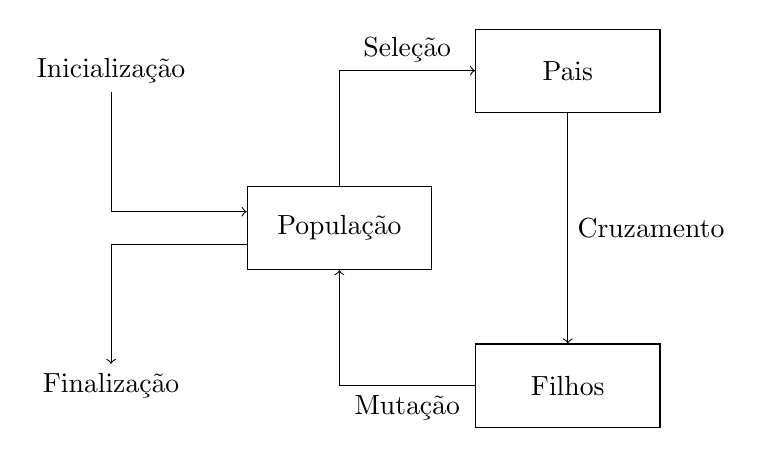
\begin{tikzpicture}[node distance = 2.9cm]
        \tikzstyle{frame} = [rectangle, draw, text width=6em, text centered, minimum height=3em]
        \tikzstyle{line} = [draw, ->]
        \node [frame] (pop) {População};
        \node [above=2cm, left of=pop] (init) {Inicialização};
        \node [below=2cm, left of=pop] (term) {Finalização};
        \node [frame, above=2cm, right of=pop] (parents)  {Pais};
        \node [frame, below=2cm, right of=pop] (off)  {Filhos};
        \path [line] (parents) -- node[right,align=left,pos=.5] {Cruzamento}(off);
        \path [line] (init) |- (pop.170);
        \path [line] (pop.190) -| (term);
        \path [line] (off) -| node[below,pos=.25, align=center] {Mutação}(pop);
        \path [line] (pop) |- node[above,pos=.75, align=center] {Seleção}(parents);
    \end{tikzpicture}
    \caption{Processo geral de um algoritmo genético}
    \label{fig:ea_flowchart}
\end{figure}


\section{Redes Neuronais}\label{sec:neural_nets}

As Redes Neuronais Artificiais (ANNs) são modelos computacionais inspirados no funcionamento do cérebro humano, compostos por unidades de processamento, chamadas neurónios, responsáveis por receber entradas, processar informação e gerar saídas.
As ANNs utilizam conexões sinápticas ajustáveis para aprender com os dados de entrada~\cite{Lippmann1988AnNets}.

Essas redes possuem a capacidade de aprender por meio de exemplos e generalizar esse conhecimento para novos dados.
Por essa razão, elas são amplamente utilizadas em diversas áreas, como reconhecimento de padrões, classificação, previsão, processamento de imagens, entre outras~\cite{Jain1996ArtificialTutorial}.

Atualmente, as ANNs são consideradas ferramentas fundamentais para aprendizagem de máquina (ML) e inteligência artificial (AI), com inúmeras aplicações práticas em saúde, finanças, indústria e outros setores.


\section{Otimização de Redes Neuronais}\label{sec:optim_nns}

A crescente popularidade das ANNs na década de 80 potenciou o surgimento de novas técnicas para o seu treino e otimização, com particular atenção para os algoritmos genéticos.
A retropropagação (BP), apesar da sua utilidade e simplicidade, apresentava limitações, entre as quais:
\begin{itemize}
    \item a pobre escalabilidade face ao aumento da complexidade do problema (maior dimensionalidade e/ou complexidade dos dados), resultando numa degradação de desempenho;
    \item a necessidade de diferenciabilidade no cálculo dos gradientes, que impede o seu uso em certos tipos de nós e critérios de otimização não diferenciáveis.
\end{itemize}

Para superar essas limitações, Montana e Davis~\cite{Montana1989} propuseram um algoritmo genético capaz de codificar os pesos duma rede neuronal \textit{feed-forward} (FNN) numa lista de números reais, utilizando uma função de \textit{fitness} para avaliar o desempenho da rede, e incorporando operadores de mutação, cruzamento e gradiente para gerar novas soluções.

Montana e Davis realizaram múltiplas experiências usando uma base de dados de imagens de energia acústica, e compararam o desempenho do algoritmo genético com o da retropropagação.
Os resultados mostraram que o GA superou o BP em termos de velocidade de treino e capacidade de lidar com tipos de nós e critérios de otimização, provando os GAs como uma alternativa eficaz à retropropagação, especialmente em problemas complexos e não diferenciáveis.